\documentclass{article}

% Environment setup

\usepackage[
    margin=.75in
]{geometry} %geometry (sets margin) and other useful packages 
% \setlength{\oddsidemargin}{.25in}
% \setlength{\evensidemargin}{.25in}
% \setlength{\textwidth}{6in}
% \addtolength{\topmargin}{-0.4in}
% \setlength{\textheight}{8.5in}
\setlength{\parindent}{0em}
\setlength{\parskip}{.75em}

\usepackage{graphicx}
\usepackage{grffile}  % support extra dots in filenames
\usepackage{fancyref}
\usepackage[labelfont=bf]{caption}
\usepackage{subcaption}
\usepackage{siunitx}


\title{\textbf{CS 4460:} Project 5}
\author{Bradley Reardon (Group 43)}
\date{April 21, 2019}

\begin{document}
  \maketitle

  \section{Data}
    The data set chosen for this assignment as the aircraft incident report database, pulled from the website of the National Transportation Safety Bureau (NTSB). The data set includes nearly 2000 cases of incidents reported between 1995 and mid-2016. Each case is described by a date, aircraft make and model, and various characteristics describing the serverity of the incident, the phase of flight in which it occurred, the location, and the number of survivors, injured, and fatalities on board.

    Note that quite a few cases in this data set contained null values for some or most columns. As a result, this visualization project does rely on filtering null values for some visualizations.

  \section{Design}
    When first looking into the data set, my pre-existing knowledge of aviation triggered interest in specific fields of the data -- namely the phase of flight, the weather conditions, and overall severity of the damage. My goal was not to prove any specific point, but rather to make interesting queries about the data overall and find answers to cursory questions that could spawn deeper questions about the data. Because the data set is only for reported incidents and does not contain information about the frequency of certain models of aircraft being flown, it is difficult to make any specific determinations, for example, for a question such as ``what is the most dangerous aircraft to fly'', as that would require an ``incidents per flight hour'' metric of some sort.

    In addition, I aimed to explore different types of visualizations and interactions with the visualization in order to effectively summarize and categorize data into simple, easy-to-understand formats. Rather than creating an elaborate view with many actions, filters, brushes, or so on, I chose to create simpler visualizations as part of an overall narrative. My goal in this was to communicate some sort of story and interject knowledge from outside of the data set to make the data speak better for itself.

  \section{Analysis}
    This visualization project supports multiple analytic tasks on the data used. Each visualization aims to provide an overview for a basic question. The first visualization narrows incidents down to the top 20 for two categories to keep the most significant data in view. In addition, the third visualization provides an overview of the most critical phases of flight in which incidents occured, in order to narrow down the number of distinct phases of flight that a user would have to look through.

    The third visualization is simple in view in order to allow a user to only see the details on demand that they are interested in. The first visualization shows more detail when bars are hovered over, in order to allow the user to relate the data for aircraft models in the two side-by-side charts with each other, as well as to see a total fatality number that is not otherwise shown in the chart.

    Finally, the second visualization summarizes substantial damage events among aircraft and allows the user to view all data at once, then zoom into particular time periods at will.

  \section{Implementation}
    The main goal with the implementation of the visualization UI was to use a storytelling narrative similar to an interactive visualization one may find from a news organization website. With this, a simple monotone design with greys was selected for the main color scheme of the page, with each of the visualizations using different colors to provide visual distinction between categories and rank.

    \Fref{fig:v1} shows the first visualization. This visualization focuses on providing side-by-side bar charts for two separate analytical questions regarding total reported incidents, as well as incidents that resulted in a destroyed airframe. Hovering over each bar shows a tooltip, reporting total fatalities as well as incidents and destruction events.

    \begin{figure}[htb]
      \centering
      \frame{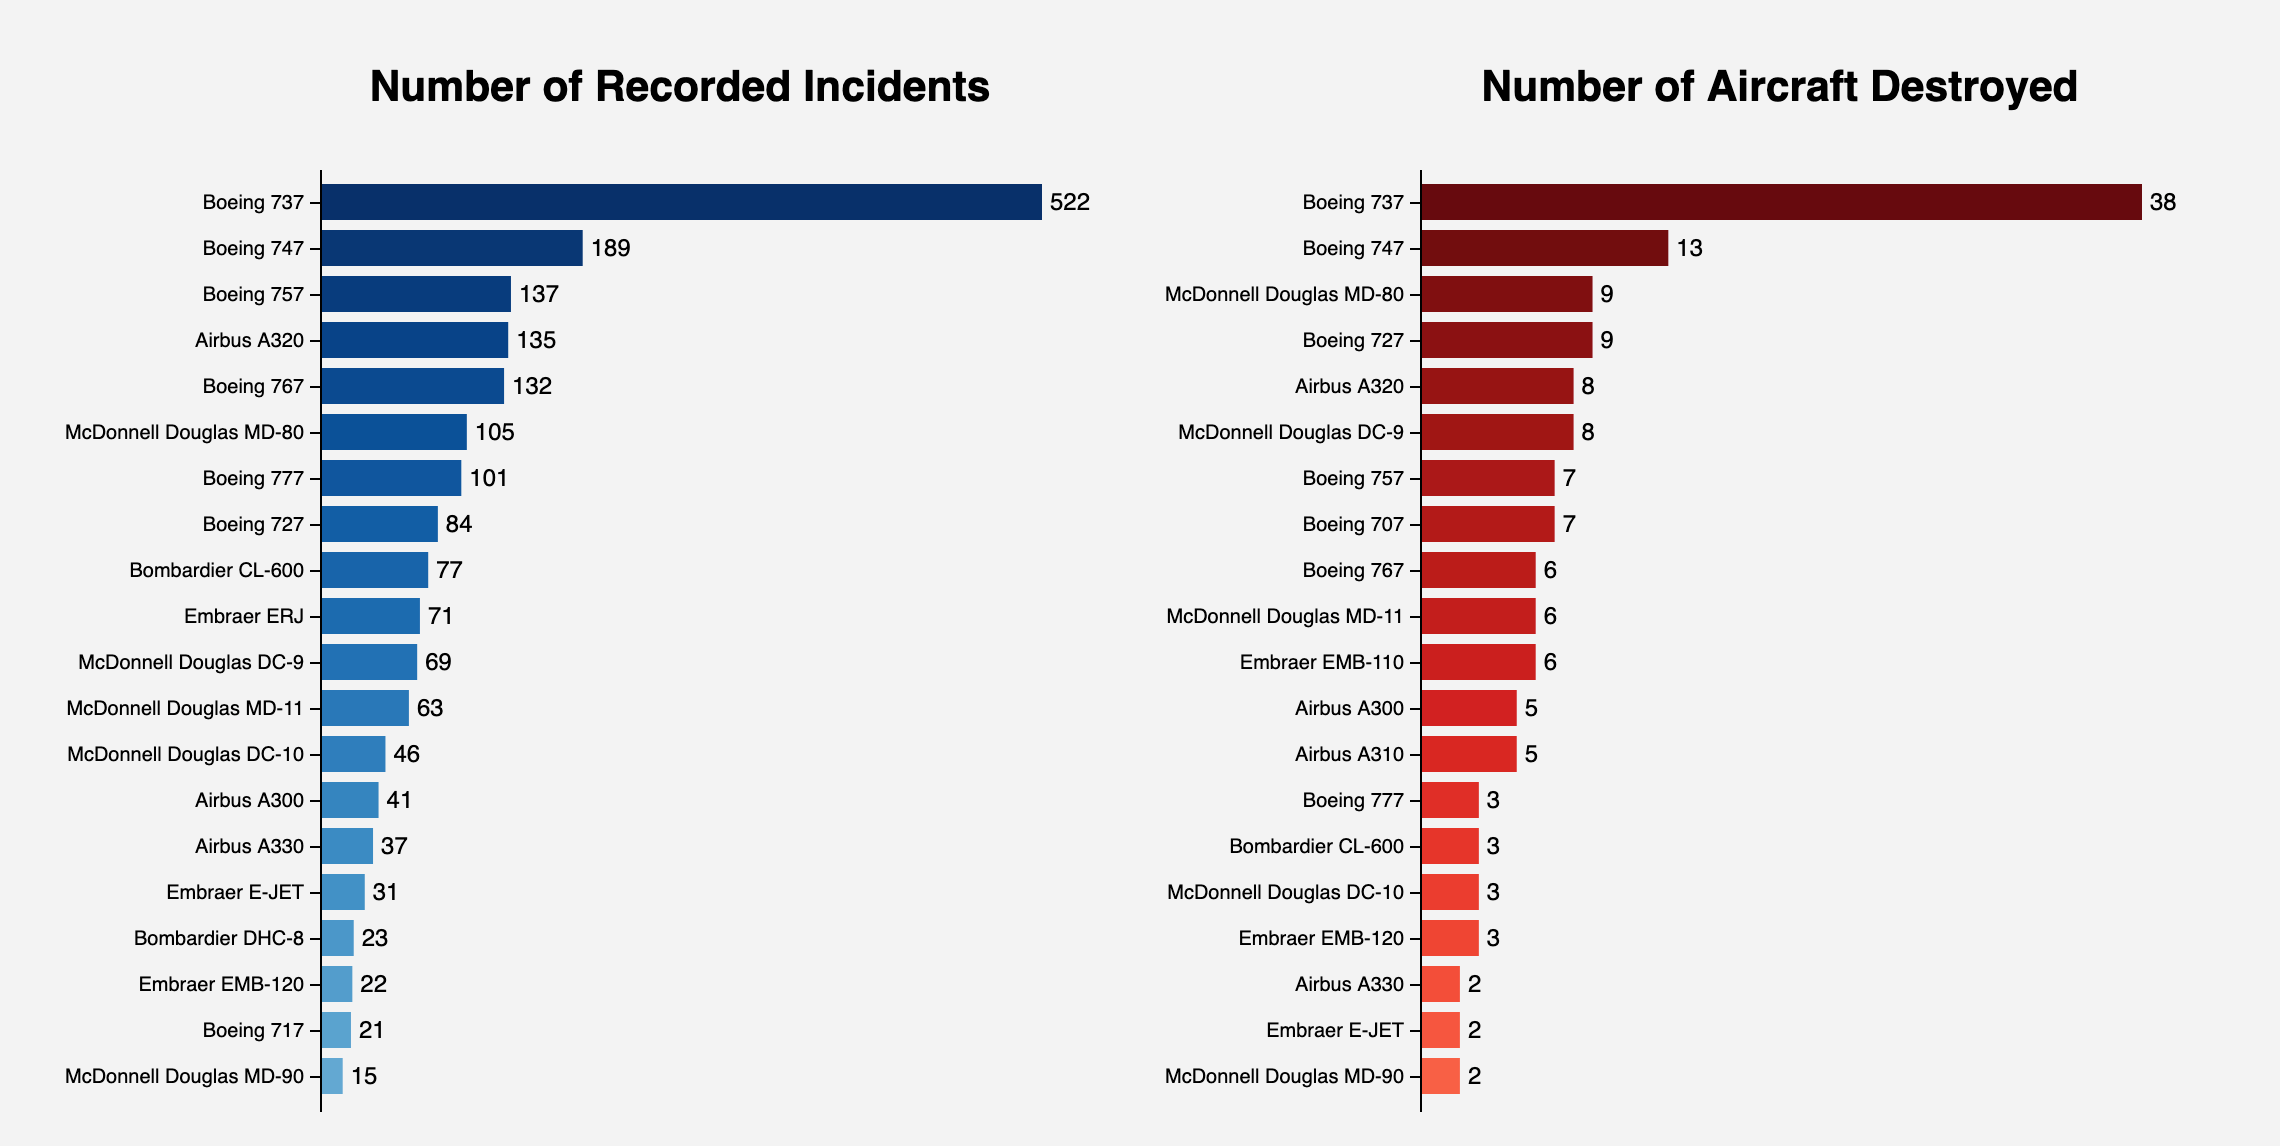
\includegraphics[width=.8\linewidth]{fig/v1}}
      \caption{Visualization 1, focusing on total incidents per aircraft model and total destroyed aircraft per model.}
      \label{fig:v1}
    \end{figure}

    \Fref{fig:v2} shows the second visualization, which is a histogram of substantial damage events through the breadth of the data set. This histogram allows zooming and panning via the scroll wheel to allow the user to drill down to specific time periods and assess the safety of aircraft over time.

    \begin{figure}[htb]
      \centering
      \frame{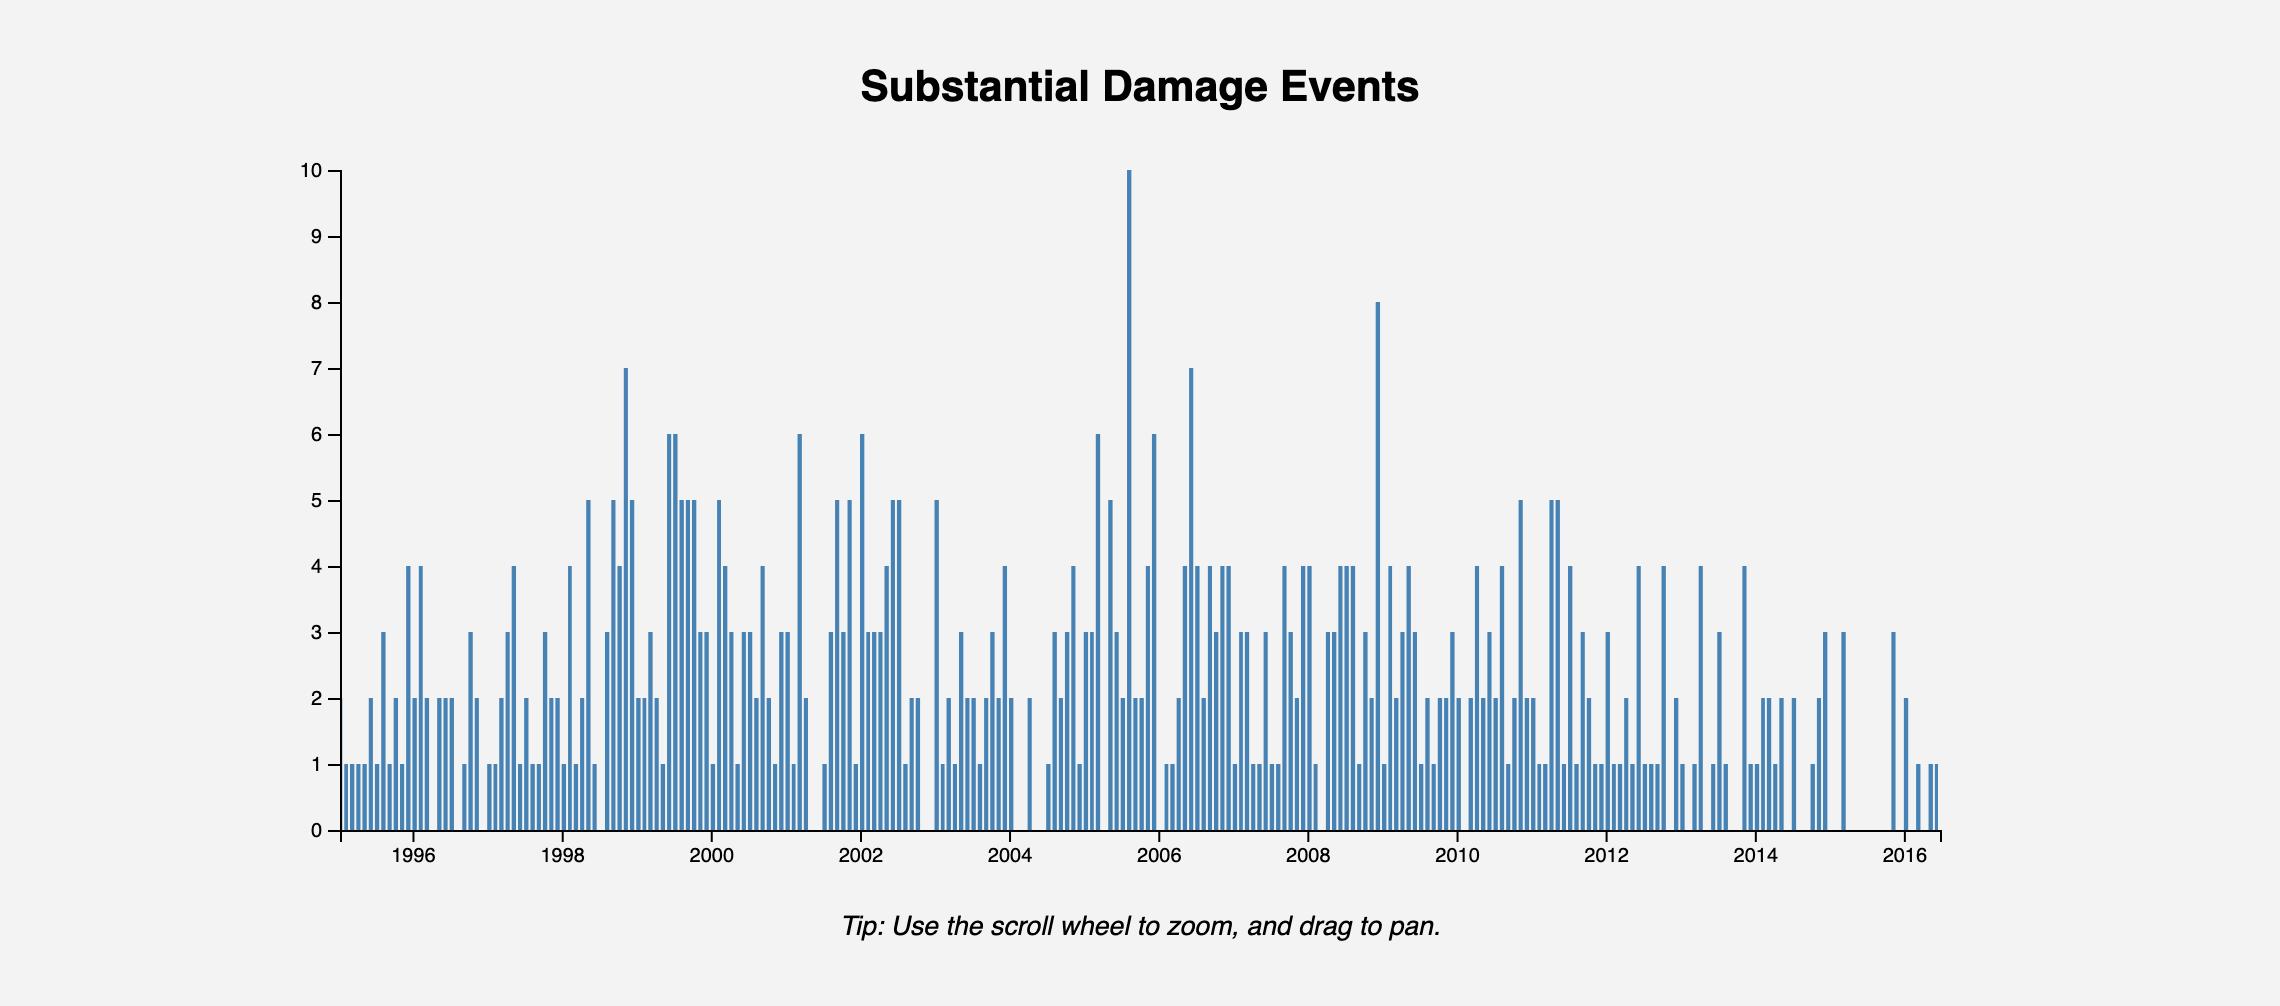
\includegraphics[width=.8\linewidth]{fig/v2}}
      \caption{Visualization 2, showing a time series histogram binning substantial damage events per month over the whole data set.}
      \label{fig:v2}
    \end{figure}

    \Fref{fig:v3} shows the third and final visualization, which provides insight into the weather conditions at the time of incidents with reported weather. Each donut chart in this visualization shows the main 5 critical phases of flight, along with an other category, to illustrate which phases of flight during which incidents most often occured in either visual meteorological conditions (VMC; good flying weather) or  instrument meteorological conditions (IMC; poor flying weather).

    \begin{figure}[htb]
      \centering
      \frame{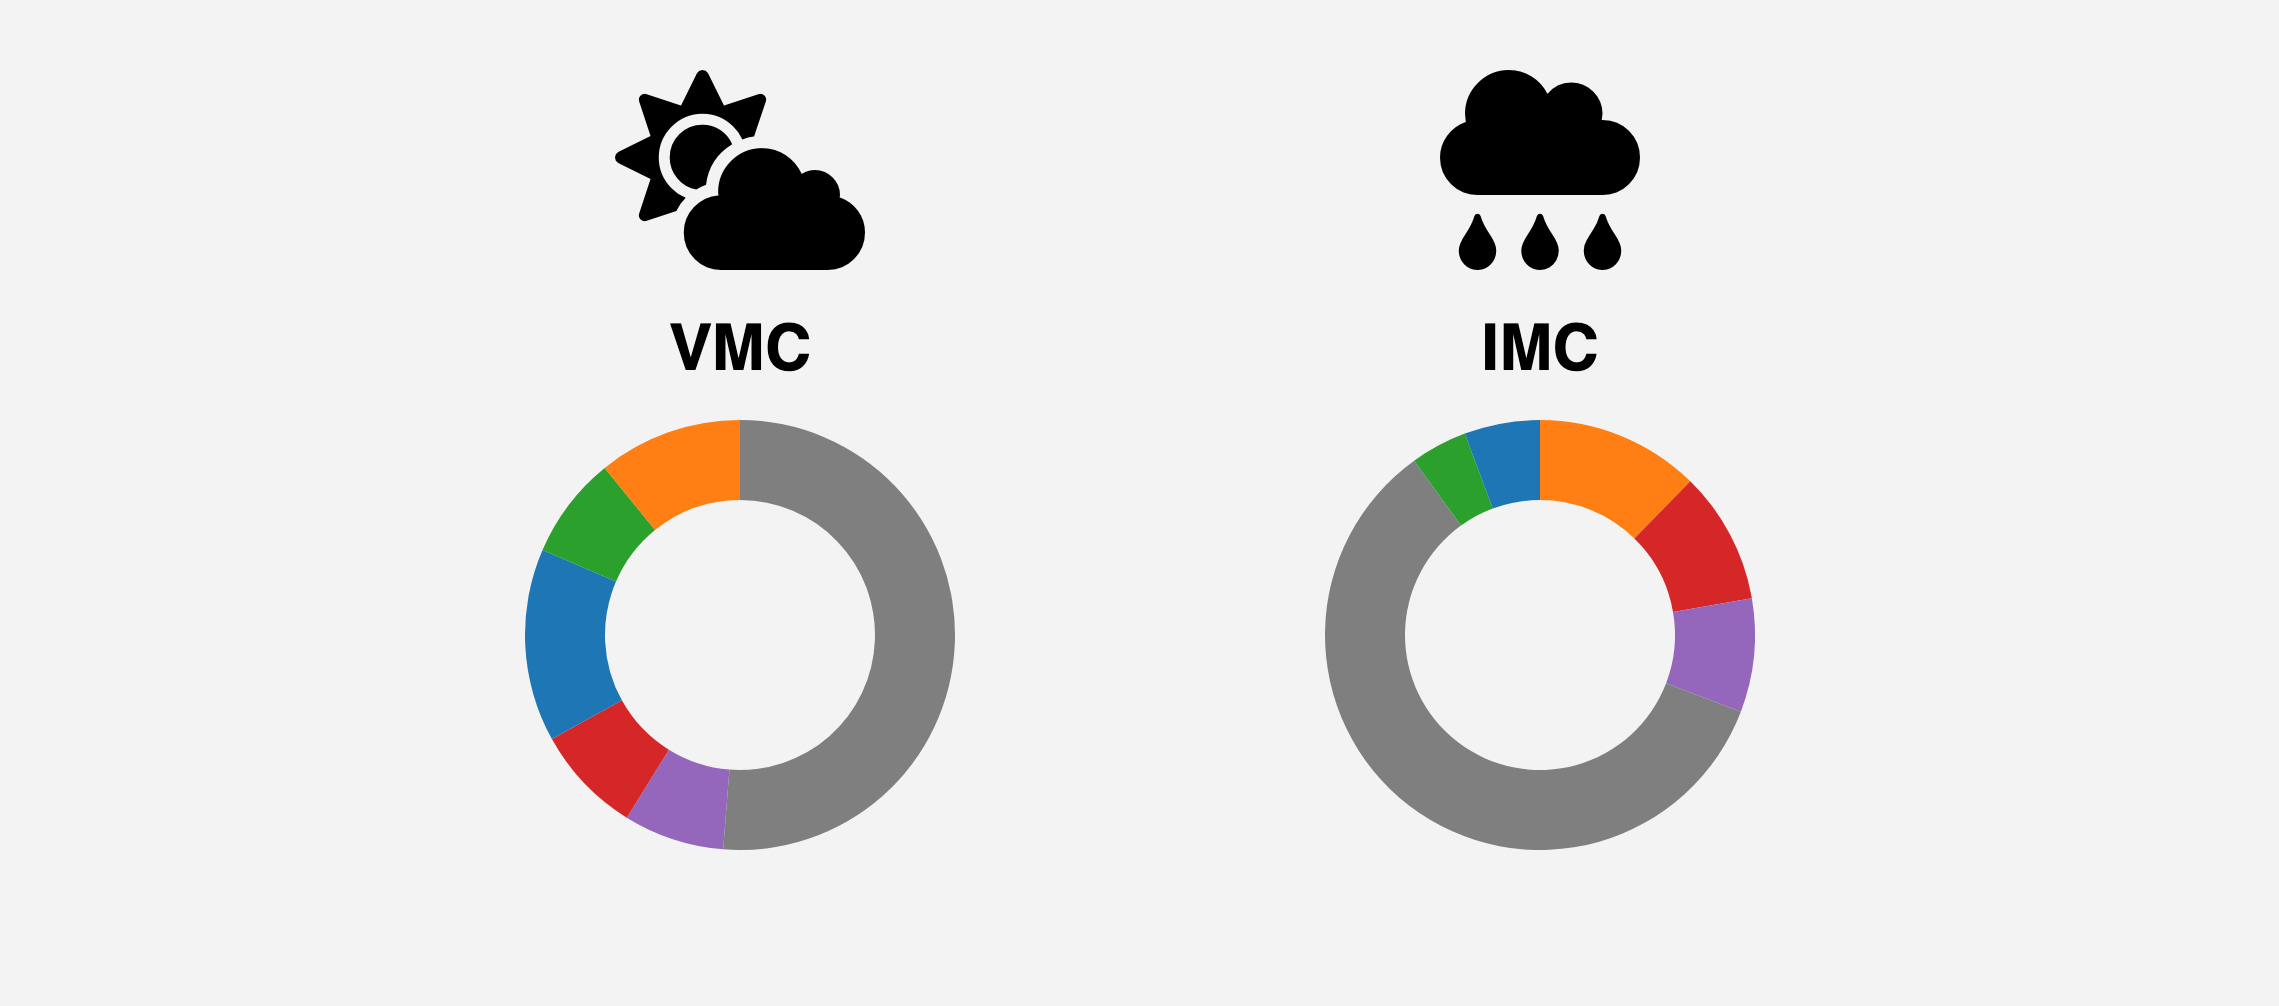
\includegraphics[width=.8\linewidth]{fig/v3}}
      \caption{Visualization 3, a donut chart allowing the user to hover and show total incidents per phase of flight for good and bad flying conditions.}
      \label{fig:v3}
    \end{figure}

  \section{Conclusion}
    The end goal of this project was to produce a series of visualizations that allow a reader to synthesize deeper questions about the aircraft incident data explored in this project. By no means does this website function as a complete data visualization tool. However, given other data sources and statistics, perhaps this website could answer some deeper questions about the data that otherwise would remain unanswered.

    Mainly, the challenges of parsing location data from the many forms provided in the data set were out of scope for this project, but future explorations of these topics would likely lead to more visualizations with geographical data and better time series visualizations as well.

\end{document}